\begin{tikzpicture}
	%\draw[help lines] (0,0) grid (6,4);
	\begin{axis}[axis lines=middle, axis equal, grid=both, xlabel = $\operatorname{Re}$, ylabel = $\operatorname{Im}$]
		\draw (axis cs: 0, 0) circle [black!10, radius=1];
		% this uses per-patch color data:
		\addplot[patch, opacity=0.5, table/row sep=\\, patch table={%
			0 1 2\\
			1 2 3\\
			4 3 5\\
		}]
		table[row sep=\\,point meta=\thisrow{c}] {
			x		y		c	\\
			-1		0		0	\\% 0
			-0.5	0.866	1	\\% 1
			0		0 		1	\\% 2
			0.5		0.866 	0	\\% 3
			0		0 		1	\\% 4
			1		0 		1	\\% 5
		};
		\addplot[patch, opacity=0.5, table/row sep=\\, patch table={%
			0 1 2\\
			1 2 3\\
			4 3 5\\
		}]
		table[row sep=\\,point meta=\thisrow{c}] {
			x		y		c	\\
			-1		0		0	\\% 0
			-0.5 	-0.866	1	\\% 1
			0		0 		1	\\% 2
			0.5		-0.866	0	\\% 3
			0		0		1	\\% 4
			1 		0		1	\\% 5
		};
		\draw[latex-latex, red]  ([shift=(60:1cm)]110, 84) arc(0:45:1cm) node[midway, rotate=30, right, red] {$\varphi = \dfrac{2\pi}{6}$};
		\addplot[orange, very thick, mark=*] coordinates{(1, 0) (1, 0)} node[above, red!70] {$e_1^{(6)}$};
		\addplot[orange, very thick, mark=*] coordinates{(0.5, 0.866) (0.5, 0.866)} node[above, red!70] {$e_2^{(6)}$};
		\addplot[orange, very thick, mark=*] coordinates{(-0.5, 0.866) (-0.5, 0.866)} node[above, red!70] {$e_3^{(6)}$};
		\addplot[orange, very thick, mark=*] coordinates{(-1, 0) (-1, 0)} node[above, red!70] {$e_4^{(6)}$};
		\addplot[orange, very thick, mark=*] coordinates{(-0.5, -0.866) (-0.5, -0.866)} node[above, red!70] {$e_5^{(6)}$};
		\addplot[orange, very thick, mark=*] coordinates{(0.5, -0.866) (0.5, -0.866)} node[above, red!70] {$e_6^{(6)}$};
		\addplot[->, dashed, white] coordinates{(0.8, 1.1) (0.8, 1.2)}; % for axis-scaling
		\addplot[->, dashed, white] coordinates{(0.8, -1) (0.8, -1.2)}; % for axis-scaling
	\end{axis}
\end{tikzpicture}